% Chapter 1

\chapter{Introduction} % Main chapter title

\label{Chapter1} % For referencing the chapter elsewhere, use \ref{Chapter1} 


\section{Objective}


This study's motivation originates from the wealth of offshore wind developments in the United States (US) East Coast during recent years. The Bureau of Offshore Energy Management (BOEM) has already leased several areas between the coastal and continental shelf limits that correspond to multiple projects to construct and manage offshore wind farms. BOEM has recently released a guideline addressing the oceanographic and meteorological conditions that need to be characterized to support the offshore wind farms' infrastructure development \cite{DNVGL2018}. Wind and wave conditions are two of the leading environmental factors connected to offshore wind. Their accurate estimation is crucial for the design, the operation, and the energy yield of an offshore wind facility.

There is a need for long-term and reliable data records to estimate the wind and wave conditions. Numerical models and observations support offshore wind energy with the characterization of these conditions. There are two primary objectives of good quality observations. On the one hand, they are an independent source of knowledge that we use to study the environmental conditions and climate. On the other hand, observations are used to enhance the robustness of numerical models through data assimilation. This study focuses on the Southern New England (SNE) wind and wave regime's characterization using in situ observations from buoy stations that are moored in the domain and from satellite altimeters. We take advantage of the National Data Buoy Center (NDBC) and Coastal Data Information Program (CDIP) extended network of stations for the in situ data. These observations are closer to the ground truth, but the sensors' measurements onboard buoys contain inherent sources of errors. The advantage of in situ stations is that they provide a long-term, reliable, and quality controlled time-series record. Therefore, they are suitable for the accurate estimation of the normal conditions in our area of interest. However, they represent measurements in point locations; hence, there are spatial gaps in our estimates. Observations from multiple satellite altimeters can partly fill these spatial gaps; thus, first, we aim to compare and validate altimeters with in situ data and then provide maps of the wind and sea state primary measures. The satellite altimeters' disadvantage is the low temporal resolution, as it depends on each satellite’s cycle, the period that elapses until it passes again over the same region.



\section{Study Area}\label{study_area}


The area of interest is located in the western part of the North Atlantic ocean or the East Coast of the continental United States. The region we focus on is geographically defined by the coastal Southern New England states of  Connecticut (CT), Rhode Island (RI), Massachusetts (MA) on the east, and the New York/New Jersey bight, including Long Island on the west. 


\begin{figure}[H]
\centering
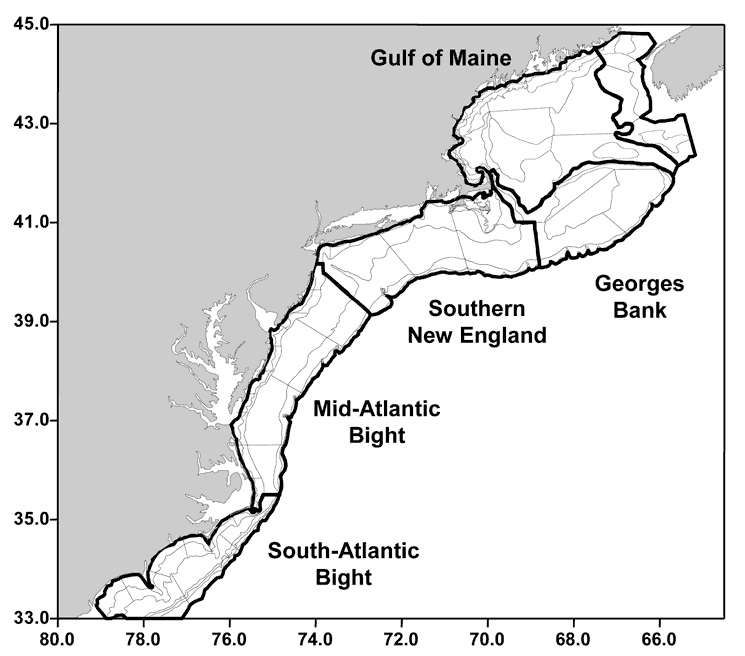
\includegraphics[width=0.85\linewidth]{Figures/Chapter1/Northwest_Atlantic_coast.jpg}
%\decoRule
\caption{US coastal regions of the Northwest Atlantic.}
\label{fig:northwest_atlantic}
\end{figure}

Specifically, the domain of interest is limited between $74^{\circ}$W and $69^{\circ}$W longitude and $39^{\circ}$N and $42^{\circ}$N latitude. Besides, it extends about 200 kilometers offshore, on the limits of the US continental shelf. 
The whole domain is referenced herein as Southern New England (SNE) for reader’s convenience, even though it contains parts of New York and New Jersey, and it is shown in Figure~\ref{fig:northwest_atlantic}.

SNE is also the birthplace of offshore wind in the United States, with Block Island wind farm being the first constructed and operating in US coastal waters \cite{Neill2018}. This region is strongly connected with offshore wind energy as many promising projects currently exist, and multiple areas shown in Figure~\ref{fig:boem_lease} have already been leased. Similar developments will also occur in the region's central and western parts soon, as BOEM has also recommended several lease areas.

The strong presence and increased frequency of extratropical storms also characterize SNE's coastal zone \cite{Vose2014}. These low-pressure systems are noticeable primarily during the fall, winter, and spring seasons. They develop in Southern latitudes, and the maximum of their intensity is often attained in the New England region. They are called Nor'easters due to the coastal wind's direction during their passing. Their impact on the coastal zone is significant as they cause high winds, extreme waves, storm surges, and coastal flooding. The maximum Wind Speed (WS) values during Nor'easters do not approach those during the passing of hurricanes. However, they are frequent over New England, and the coupling of high waves and long duration may have a minimal to a catastrophic impact on the whole region \cite{DOLAN1992}. Coastal fronts are also a common feature of late fall, early winter New England weather. Their genesis and formation close to the coast due to land-ocean differential heating or inland due to differential heating connected with the uplifting of moist air when approaching the Appalachian mountains is documented in detail in the literature \cite{Nielsen1989}.

\begin{figure}[H]
\centering
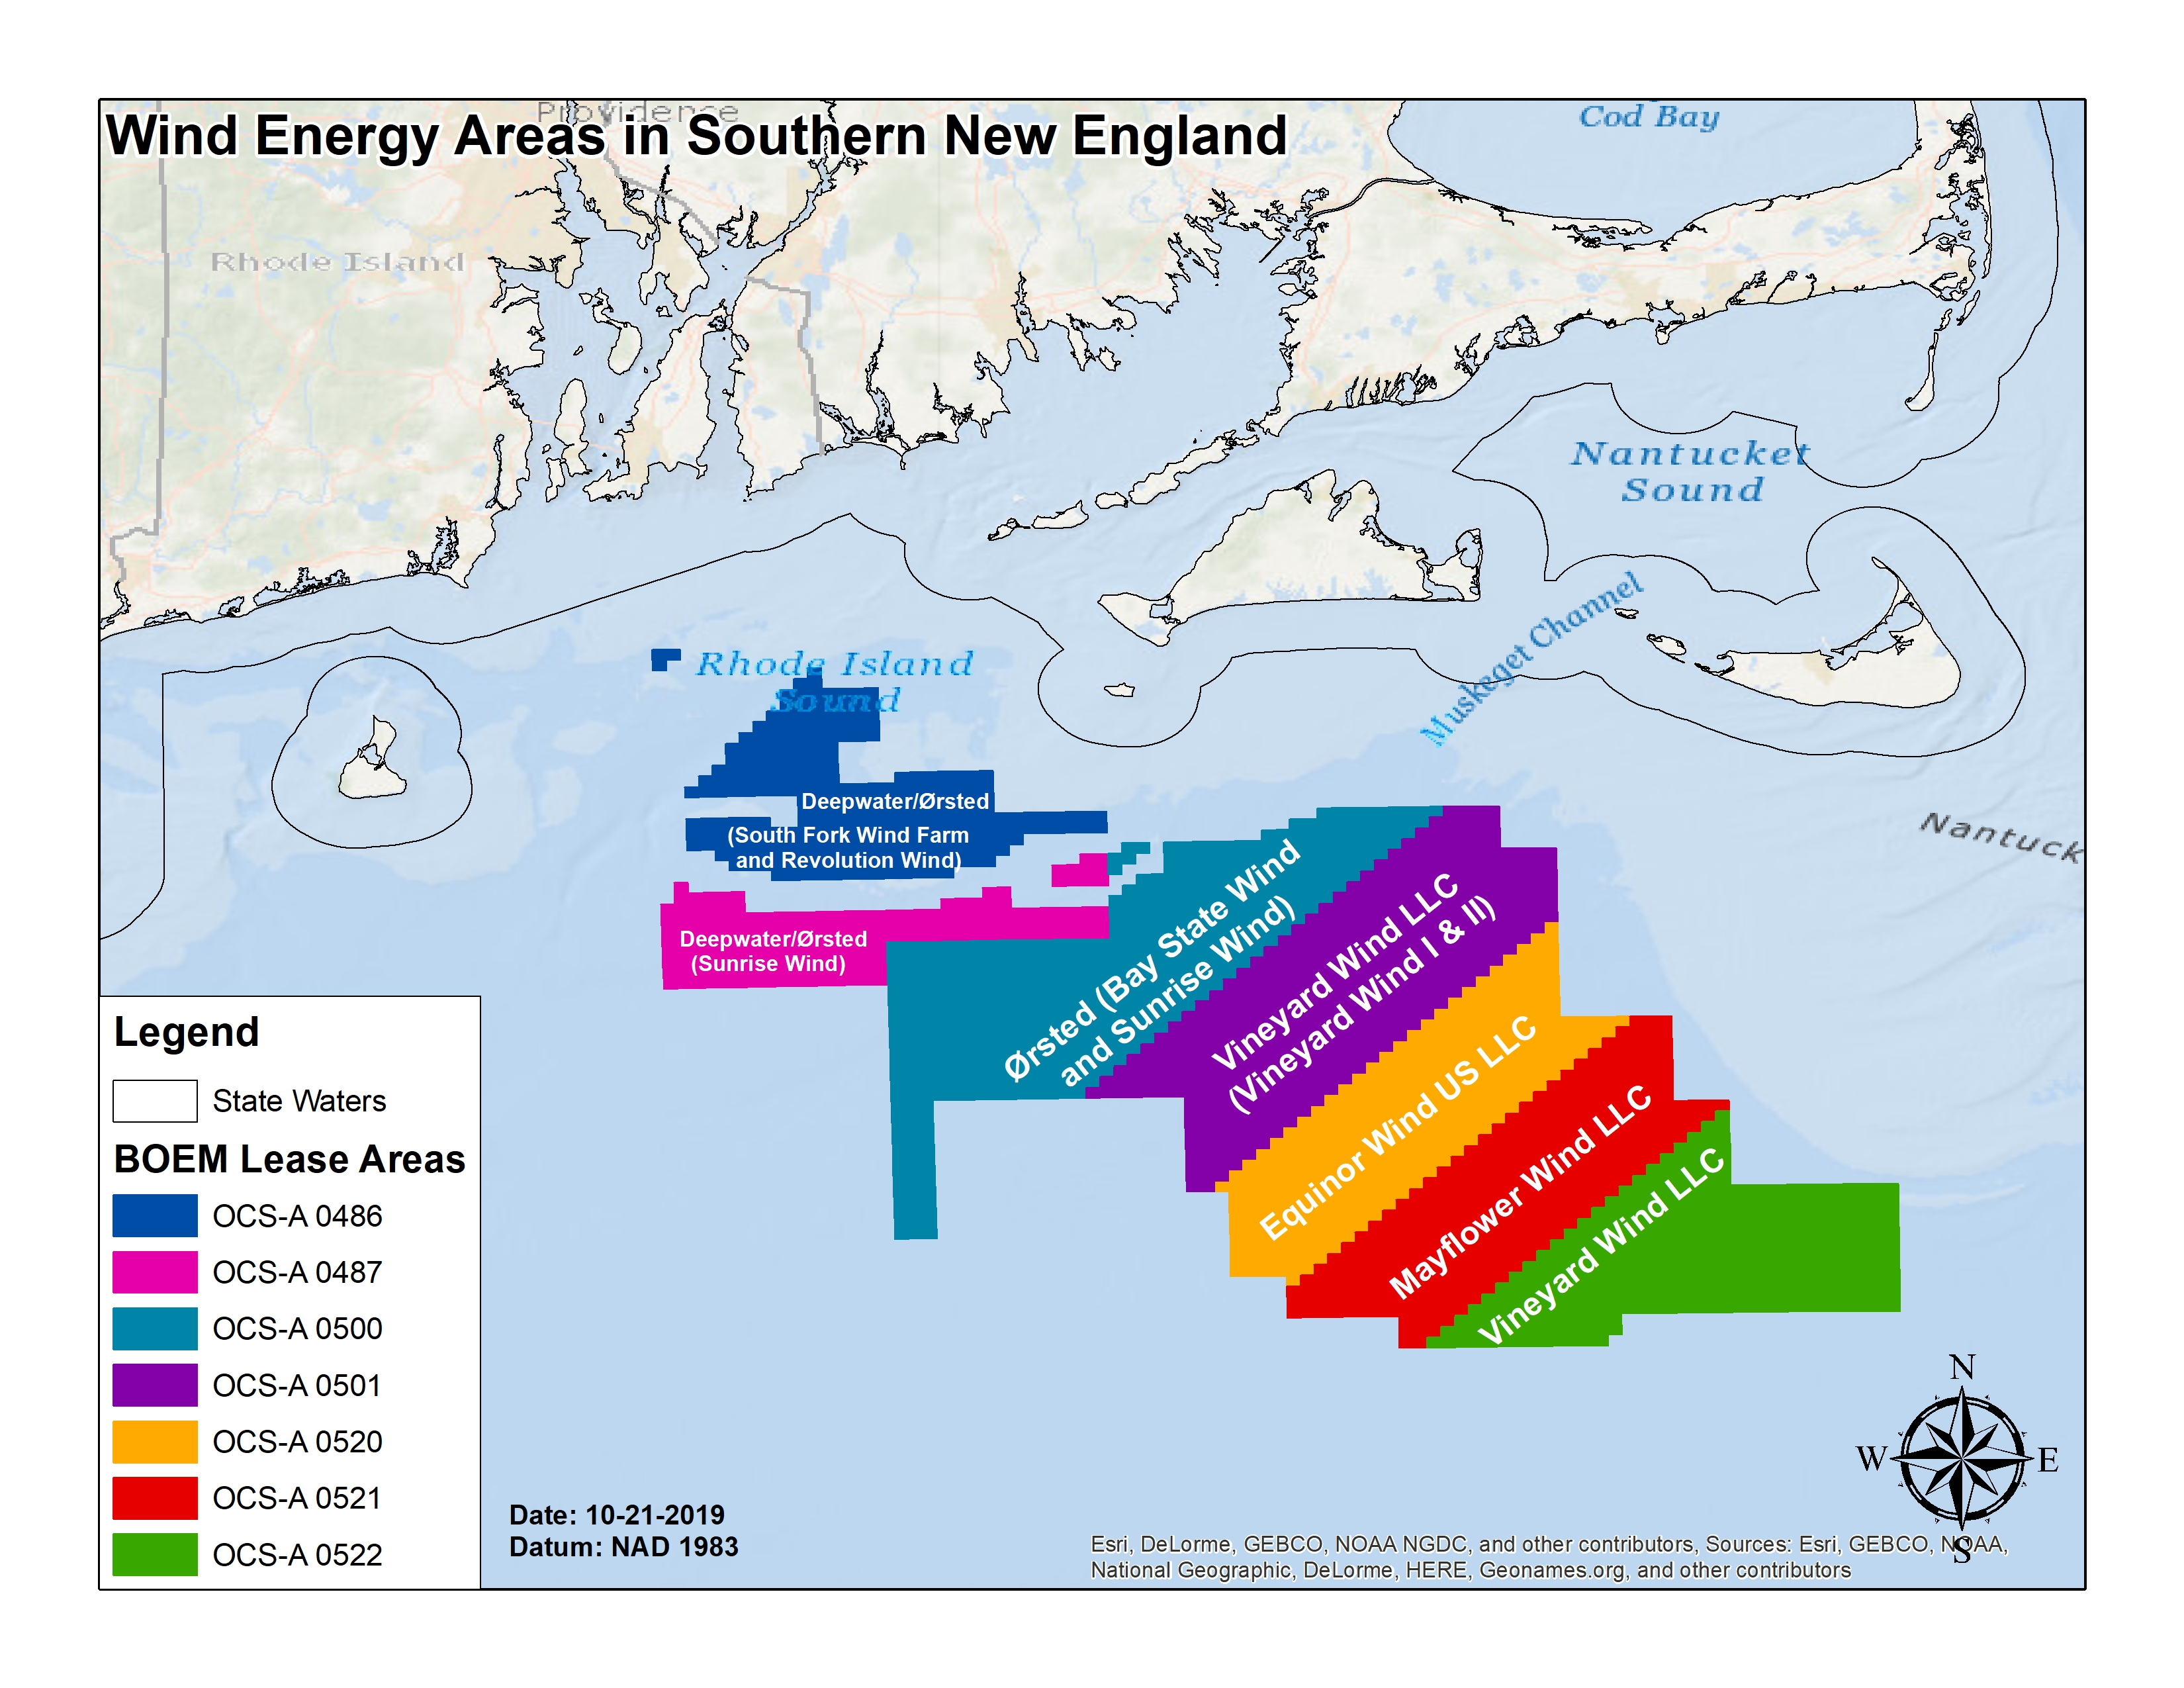
\includegraphics[width=0.95\linewidth]{Figures/Chapter1/WEAs_Map.jpg}
%\decoRule
\caption{BOEM Offshore Wind lease areas in SNE. Source: \href{http://www.dem.ri.gov/programs/marine-fisheries/images/WEAs_Map.jpg}{RI Department of Environmental Management (DEM)}}
\label{fig:boem_lease}
\end{figure}



\section{Outline}


Chapter 2 provides the theoretical background of this study. First of all, we define the wave parameters reported from in situ and remote sensing observations. One of the common parameters often used to characterize the sea state is the Significant Wave Height (SWH). We examine how it is connected with the directional wave spectra and how it is derived from it. One of the several ways to take advantage of the directional spectrum of waves leads us to review the different ways to separate the sea states, a process called spectral decomposition. An alternative way to empirically separate the sea states based on their growth stage is by considering their wave age, which connects the wave speed of propagation with the WS. Besides, a literature review of the bulk formulas used historically to connect the WS, and SWH is provided, examining their limitations. Bulk formulas are also used to estimate the waves’ interaction with the wind over the ocean. The unavailability of multiple parameters required for the accurate description of the boundary layer's stability is often a limitation. Therefore, due to these restrictions, we often use the wind speed profile over the ocean and the governing laws of air-sea interaction with assumptions of the conditions near the sea surface. The wind speed probability density functions (PDFs) are essential to estimate the mean wind power density close to the offshore wind planned area. Studies connected with offshore wind research include estimating the PDF parameters and searching for innovative ways to select the optimal PDF to characterize the wind speed distribution. We provide the four distributions and their theoretical PDFs with the best fit for the SNE region's data. Finally, data from satellite altimeters are measured with entirely different methodologies than those used for in situ observations. They also represent different spatial and temporal scales of the wind and wave conditions. Therefore, the principles of satellite altimetry are described to explain these differences.

Chapter 3 includes a detailed description of the methodologies used to derive our results. An integral part of all the studies that include observations is data preprocessing. It consists of the collection, organization, and description of the various datasets used. The accuracy of the measurements and the detection of error sources are also essential to filter out erroneous data. All the above are provided both for the buoy and the satellite altimeter observations. A spatiotemporal collocation methodology is required to validate altimeter observations' consistency with respect to in situ, which are considered the ground truth reference. A description of the limitations of such comparisons is also provided. After validating the satellite altimeter observations, variogram modeling is used to describe the observations' spatial correlation. This process is critical for interpolation to create maps of the WS and SWH spatial variability and estimate the predictions' uncertainty.


Chapter 4 contains all the results. The first section is about the wind and wave climatology of the SNE based on  buoy data. We examine different temporal scales of variability, including the diurnal, seasonal, and interannual, for each buoy with an available long-term record. The goal is to define the normal wind and wave conditions in SNE. The wind and wave directional characteristics are also of high importance. Hence, we provide and visualize the directional distribution of WS and SWH. We also emphasize the benefits of considering the directional wave spectra for a detailed description of the wave climate. The WS and SWH relationships are estimated using polynomial regression analysis. The differences between these relationships with respect to wind direction are also examined for each location. The classification of waves is performed based on their inverse wave age. An extreme event is analyzed and described as a case study. The parameters of WS PDFs that best fit the data from individual stations are estimated and evaluated. Validation of the data from multiple satellite altimeter missions is performed using buoy observations as a reference. An evaluation of their performance is also included. Satellite altimeter data are interpolated for recent winter and summer seasons to estimate the wind and wave spatial distribution in the SNE region. The limitations of this process are discussed. The impact of including data from multiple satellite altimeters on the estimation errors is also assessed.


Finally, Chapter 5 summarizes the results, including the scientific questions raised from this study to motivate future related research.



%----------------------------------------------------------------------------------------

% Define some commands to keep the formatting separated from the content 
\newcommand{\keyword}[1]{\textbf{#1}}
\newcommand{\tabhead}[1]{\textbf{#1}}
\newcommand{\code}[1]{\texttt{#1}}
\newcommand{\file}[1]{\texttt{\bfseries#1}}
\newcommand{\option}[1]{\texttt{\itshape#1}}

%----------------------------------------------------------------------------------------



%----------------------------------------------------------------------------------------
